\chapter{Construção da ontologia}

  \section{Protégé}

      
  O Protégé é uma ferramenta que permite a construção de ontologias de domínio, como também, a personalização de formulários
  de entrada de dados e inserção e edição de dados,  possibilitando assim, a criação de bases de conhecimento guiadas por ontologias.
  \cite{semprebom07}
  
  Para a construção da ontologia deste projeto, foi utilizada a versão (3.1) do Protégé. A Figura \ref{fig:interface_protege} ilustra
  a interface gráfica da ferramenta, que prôve acesso a ferramentas e menus, além de cinco áreas de vizualização (\textit{views}) que 
  se comportam como módulos de navegação e edição de classes, atributos, formulários e instâncias, propiciando entrada de dados,
  recuperação das informações e pesquisas na base de conhecimento. \cite{semprebom07}
  
  \begin{figure}[h] 
    \centering 
    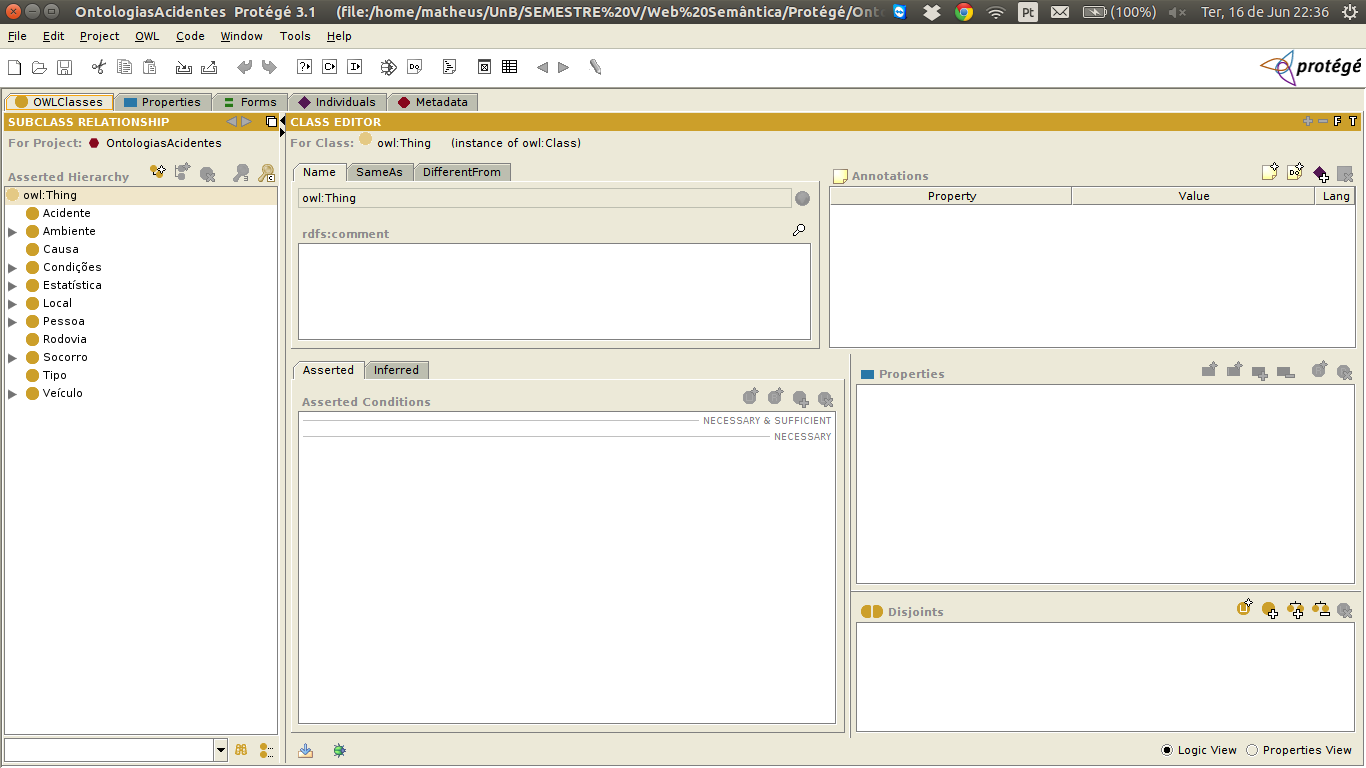
\includegraphics[scale=0.3]{interface_protege} 
    \caption[Interface gráfica do Protégé]
    {Interface gráfica do Protégé}
    \label{fig:interface_protege}
  \end{figure}
  
\subsection{Características do Protégé}

  Esta seção apresenta algumas características da ferramenta Protégé que estão listadas abaixo: 
  (\citeauthor{semprebom07}, \citeyear{semprebom07} \textit{apud} \citeauthor{freitas04}, \citeyear{freitas04}).
  
  \begin{itemize}
    \item A linguagem PAL (\textit{Protégé Axiomatic Language}, uma linguagem axiomática, permite a inserção de restrições e axiomas
    que incidem sobre classes e instâncias pertencentes a uma ou mais ontologias;
    \item A ferramenta provê a geração de arquivos de saída alteráveis, onde podem ser criadas classes e instâncias em CLIPS (motor 
    de inferência) - a base de conhecimento é gerada nativamente para esse motor.
    \item Interface para entrada de conhecimento, com um gerador automático de formulários para classes definidas. A reposição da interface
    original por componentes mais adequados à aplicação é admitida. A interface da ferramenta facilita, sobretudo, o gerenciamento de
    conhecimento de uma ou mais ontologias.    
  \end{itemize} 
  
      Os arquivos de saída suportados são: Jess, F-Logic, Prolog, RDF, OIL, XML, Topic Maps. \cite{semprebom07}

  \section{Metodologia utilizada para construção}
    
    
  A partir da análise conceitual dos métodos e metodologias para construção de ontologias presentes na sessão anterior, 
  o método escolhido para a realização deste projeto, levando em conta as etapas/fases propostas por cada uma dessas 
  metodologias ou métodos no que tange ao processo de construção de ontologias, foi o método \textit{\textbf{Ontology 101}}.
  
  Os aspectos observados na escolha do método foram: \textbf{a)} suporte literário bem consolidado e disponível 
  (livros, artigos, guias e etc); \textbf{b)} o método é baseado na literatura do paradigma orientado a objetos;
  \textbf{c)} familiarização por parte dos integrantes do grupo com os conceitos e processos propostos pelo método.

\vspace{0.5cm}
  
{\raggedright
  \textit{\textbf{Ontology 101}}.
}
  
  De acordo com Breitman (\citeyear{breitman05}), o processo de construção de uma ontologia a partir do método 101,
  resumidamente, envolve as seguintes etapas:
  \begin{itemize}
   \item Definição das classes dessa ontologia;
   \item Disposição das classes em uma hierarquia taxonômica;
   \item Definição de propriedades e valores para os mesmos;
   \item Preenchimento dos valores das propriedades para cada instância.
  \end{itemize}
  
  \begin{figure}[!htb]
    \centering
    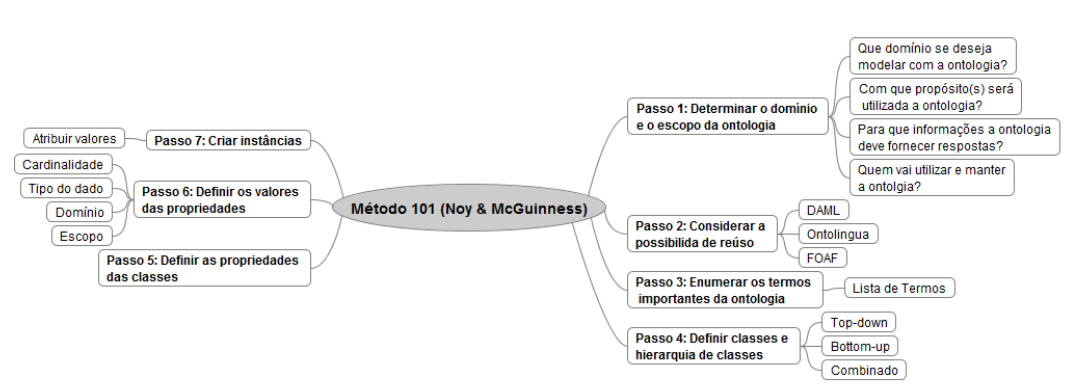
\includegraphics[scale = 0.4]{101-Web}
    \caption[Método 101 para construção de ontologia]{Método 101 para construção de ontologias. Fonte: \cite{bortolato14}}
    \label{fig:101-Web}
  \end{figure}
  
  A Figura \ref{fig:101-Web} ilustra um esquemático do método 101 no qual é detalhado cada um dos seus sete passos.
  
\vspace{0.5cm}  
  
{\raggedright  
  \textbf{1º Passo: Determinar o domínio e o escopo da ontologia}
}
  
  Para se determinar o domínio e o escopo da ontologia, Natalya F. Noy e Deborah McGuinness sugerem os seguintes questionamentos
  \cite{breitman05}:
  
  \begin{itemize}
   \item Que domínio se deseja cobrir com a ontologia?
   \item Com que protótipo(s) será utilizada a ontologia?
   \item Para que informações a ontologia deve fornecer respostas?
   \item Quem vai utilizar e manter a ontologia?
  \end{itemize}
  
  Segundo Breitman (\citeyear{breitman05}), estas perguntas servirão para avaliar a ontologia após sua conclusão.
  
\vspace{0.5cm}  
  
{\raggedright  
  \textbf{2º Passo: Considerar o reúso de outras ontologias}
}
  
  É importante considerar os termos que alguém já codificou em uma ontologia e se é possível refinar ou reutilizar
  modelos existentes para o domínio de nossa própria aplicação. Várias ontologias estão disponíveis eletronicamente,
  podendo ser facilmente importadas para editores e ambientes de desenvolvimento. \cite{breitman05}
  
  Atualmente existem várias bibliotecas de ontologias que disponibilizam modelos para reúso. As bibliotecas do projeto
  Ontolingua, DAML e KACTUS, por exemplo, disponibilizam um grande número de ontologias que podem ser reutilizadas, refinadas
  ou adaptadas. \cite{breitman05}
  
\vspace{0.5cm}  
  
{\raggedright  
  \textbf{3º Passo: Enumerar os termos importantes da ontologia}
}
  
  É útil fazer uma lista de todos os termos que deseja-se definir ou explicar aos usuários. Quais termos gostaríamos de abordar? 
  Quais propriedades terão esses termos? O que gostaríamos de dizer sobre esses termos? É importante obter uma lista compreensiva 
  de termos sem se preocupar com a redundância entre os conceitos que eles representam, relacionamentos entre termos ou qualquer 
  propriedade que eles venham a ter. \cite{noy15}
  
\vspace{0.5cm}  
  
{\raggedright  
  \textbf{4º Passo: Definir classes e a hierarquia de classes}
}
  
  Segundo Noy e McGuinness (\citeyear{noy15}), definir as classes e a hierarquia entre elas e definir  suas propriedades (5º Passo)
  são feitos de forma paralela,  pois seria difícil fazer um após o outro. O curso natural, na prática, é definir uma classe e 
  descrever suas propriedades logo após.
  
  Existem muitas abordagens possíveis para se fazer uma hierarquia de classes: \cite{breitman05}
  
  \begin{itemize}
   \item A abordagem \textbf{topo-para-baixo} (\textit{top-down}) inicia-se com a definição dos conceitos mais gerais do domínio (pai ou superclasse) 
   e, posteriormente, esses conceitos são especializados em conceitos mais específicos (filhos ou subclasses). Essa abordagem é 
   conhecida, também, como decomposição funcional. 
   \item A abordagem \textbf{baixo-para-cima} (\textit{bottom-up}), pelo contrário, inicia-se com a definição dos conceitos mais específicos 
   (filhos ou subclasses) com o subsequente agrupamento dessas classes em conceitos mais gerais (pai ou superclasse). Esses
   agrupamentos são organizados de acordo com uma estratégia de generalização. \cite{noy15}
   \item A \textbf{Combinação} (\textit{middle-out}) é a conjunção das abordagens descritas anteriormente. Primeiramente, são definidos
   os conceitos mais notórios e então esses são especializados e generalizados adequadamente. \cite{noy15}
  \end{itemize}
  
  De acordo com Noy e McGuinness (\citeyear{noy15}), nenhuma das três abordagens é a melhor a ser utilizada, isso vai depender da visão
  pessoal do modelador do domínio. Geralmente, a \textbf{combinação} tende a ser a mais utilizada pelos desenvolvedores de ontologia,
  uma vez que os conceitos mais centrais são mais descritivos no domínio da ontologia. \cite{noy15}
  
\vspace{0.5cm}  
  
{\raggedright  
  \textbf{5º Passo: Definir as propriedades das classes}
}
  
  Segundo Noy e McGuinness (\citeyear{noy15}), as classes sozinhas não proveem subsídios suficientes para responder as questões de competência
  do 1º Passo (Determinar o domínio e o escopo da ontologia). Para isso é necessário criar uma estrutura interna de seus conceitos.
  
  No passo anterior (Definir classes e a hierarquia das classes) já fora selecionadas as classes obtidas dos termos que foram listados
  no 3º Passo (Enumerar os termos importantes da ontologia).  Muito dos termos remanescentes, provavelmente, representaram as
  propriedades das classes. Para cada propriedade deve-se determinar qual(ais) classe(s) este(s) descreve(m). \cite{noy15}
  
  De acordo com Noy e McGuinness (\citeyear{noy15}), existem vários tipos de propriedades relativas a classes: intrínsecas, 
  extrínsecas, partes, relacionamentos com classes e objetos, entre outras. Todas as subclasses ou filhos de uma classe 
  (pai ou superclasse) herdam suas propriedades.
  
\vspace{0.5cm}  
\pagebreak
  
{\raggedright
  \textbf{6º Passo: Definir os valores das propriedades}
}
  
  “Propriedades podem assumir diferentes valores, dependendo da expressividade da linguagem de ontologia que está sendo utilizada”
  \cite{breitman05}. Um exemplo é a cardinalidade.
  
  Alguns sistemas permitem cardinalidade única (um único valor) entre as propriedades e ostros permitem cardinalidade múltipla 
  (propriedades multivaloradas). \cite{noy15}
  
  Na liguagem OWL, por exemplo, é permitido utilizar tipos de dados no preenchimento dos valores das propriedades. \cite{breitman05}
  
{\raggedright  
  Aqui está uma lista dos tipos de dados mais comuns:
}
  
  \begin{itemize}
   \item Cadeia de caracteres (\textit{String});
   \item Números ( Às vezes valores mais específicos de ponto flutuante (\textit{Float}) e inteiros são usados);
   \item Booleanos;
   \item Listas enumeradas de elementos.
  \end{itemize}
  
\vspace{0.5cm}  

{\raggedright  
\textbf{7º Passo: Criar instâncias}
}

  O último passo é criar instâncias individuais das classes na hierarquia. Definir uma instância de uma classe consistem em:
  (1) Escolher a classe; 
  (2) Criar uma instância individual dessa classe; 
  (3) Preencher os valores de suas propriedades. \cite{noy15}
  
    
  \section{Escopo da ontologia}
      
      A ontologia proposta neste trabalho será utilizada para o contexto de acidentes de veículos ocorridos em rodovias
      federais brasileiras, portanto, alguns conceitos inerentes a outros tipos de acidentes não se aplicam a este 
      contexto. Por esse motivo, os modelos conceituais das ontologias encontradas foram analisados e utilizados como base 
      para a construção da ontologia final.
      
      Para este trabalho, é esperado apenas uma ontologia capaz de oferecer um arcabouço mais semântico para o \textit{software} 
      "Pé na Estrada", de modo a provocar mudanças iniciais significativas no \textit{software}.
      Para trabalhos futuros, pretende-se utilizar ontologias específicas para as entidades como Pessoa, Veículo, Rodovia e
      Hospital para aumentar a representatividade da ontologia, 
      além de incluir atributos mais específicos para cada classe.
  
  \vfill
  \pagebreak
  \section{Ontologias encontradas}
   
        A fim de não ter retrabalho desnecessário, e de usar os conhecimentos previamente
  pesquisados por outros grupos de pesquisa, este grupo procurou em bases de periódicos e no
  próprio Google por ontologias que já existissem, e pudessem retratar de forma semântica os
  acidentes listados no software “Pé na Estrada”. As consultas muitas vezes não retornaram
  resultados satisfatórios, mas foi possível encontrar duas ontologias muito parecidas.
  
  De posse das ontologias, é possível observar a similaridade entre as duas encontradas,
  até por que as duas são empregadas em soluções tecnológicas parecidas. Sua aplicação
  consiste na organização das informações de acidentes em estradas, para que as informações de
  um acidente de trânsito sejam devidamente transmitidas em redes veiculares Ad hoc, ou
  VANETs \cite{barrachina12}. Essas redes usam os carros como nós de uma rede para
  trafegar informações, que podem ser analisados e registrados em banco de dados. Na
  aplicação dos projetos encontrados ela também tem a utilidade de alertar ambulâncias, ou
  hospitais próximos que possam prestar socorro de forma rápida e eficiente. As duas
  ontologias possuem as mesmas entidades e seus relacionamentos são idênticos, evidenciando
  a robustez das mesmas. A diferença está nos atributos das entidades, com a adição de diversos
  campos que fornecem informações valiosas para a correta identificação do acidente de
  trânsito \cite{villalba14}.
  
  Desta forma, as duas ontologias são tomadas como base para o contexto deste projeto,
  pois se adequam muito bem dentro dos objetivos almejados. Será proposta a adição de uma
  entidade, de forma que seja possível também captar informações sobre a rodovia a qual o
  acidente ocorreu, diferentemente da entidade ambiente (“environment”), que procura detalhar
  as condições no momento do acidente. A entidade rodovia terá atributos que irão guardar as
  informações daquela rodovia, relacionadas ao contexto do projeto. O detalhamento dessa
  entidade será conduzido no trabalho seguinte.
  
  As duas ontologias podem ser vistas na Figura \ref{fig:ontologia1} e na Figura \ref{fig:ontologia2}.
  
  \begin{figure}[!htb]
    \centering
    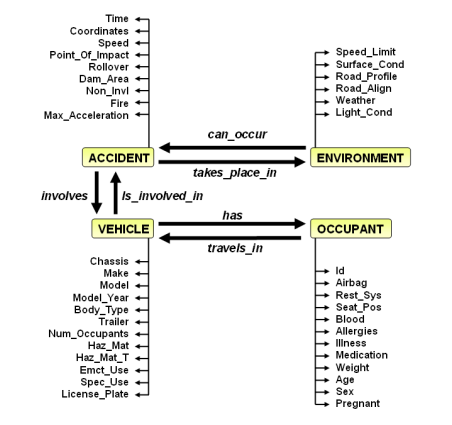
\includegraphics[scale = 0.5]{ontologia1}
    \caption[Componentes da ontologia]{Componentes da ontologia. Fonte: \cite{villalba14}}
    \label{fig:ontologia1}
  \end{figure}
  
    \begin{figure}[!htb]
    \centering
    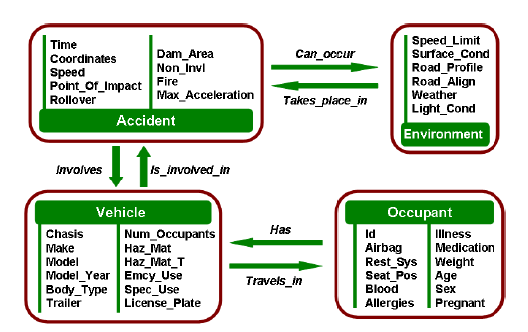
\includegraphics[scale = 0.5]{ontologia2}
    \caption[Componentes da ontologia CAOVA]{Componentes da ontologia CAOVA. Fonte: \cite{barrachina12}}
    \label{fig:ontologia2}
  \end{figure}
      
  \vfill
  \pagebreak
  \section{Estrutura da ontologia}

      Com a escolha da metodologia 101 a primeira etapa consiste na definição de classes na ontologia.
      Para essa definição foi realizada uma técnica chamada \textit{CardSorting}. A Figura \ref{fig:card_sorting} 
      ilustra os conceitos levantados pela equipe com a técnica \textit{CardSorting}.
      
      \begin{figure}[!htb]
	\centering
	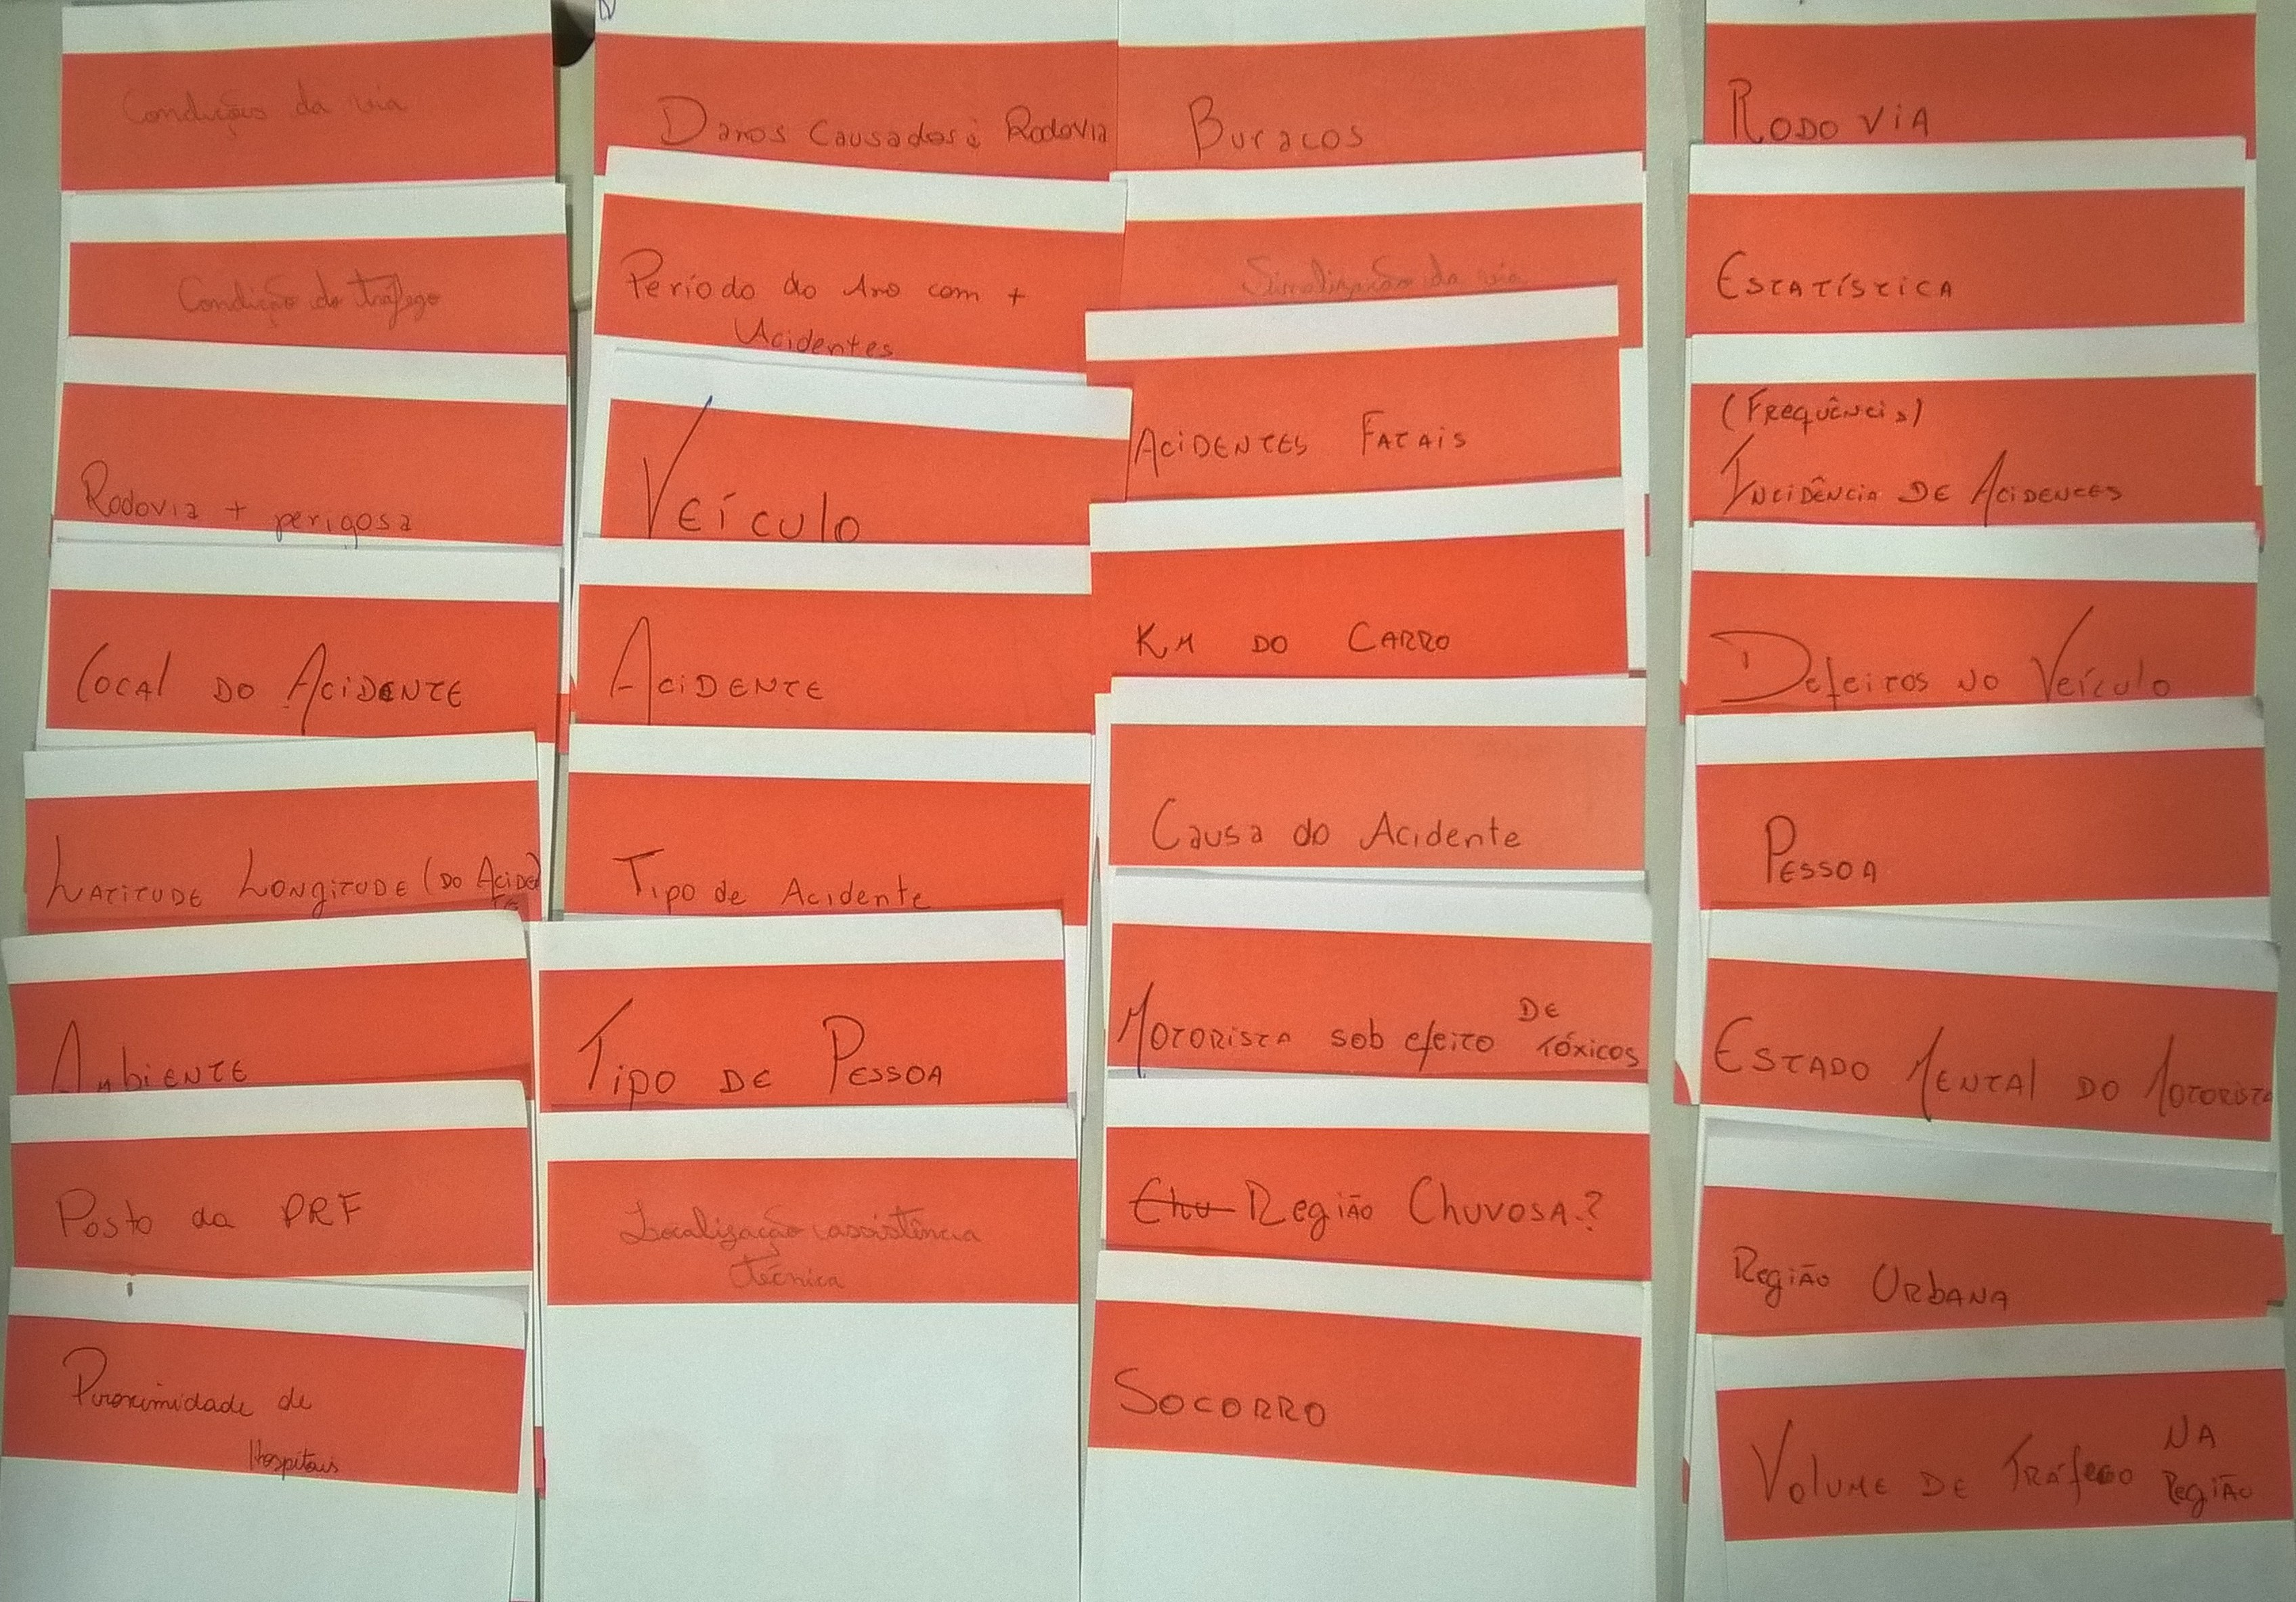
\includegraphics[scale = 0.1]{card_sorting}
	\caption[Conceitos levantados com o \textit{CardSorting}]{Conceitos levantados com o \textit{CardSorting}}
	\label{fig:card_sorting}
      \end{figure}
      
      Essa técnica consiste na escrita de termos em cartões que representem a interação do usuário com a aplicação,
      quais seriam as perguntas que ele faria ao sistema, o que ele procuraria. Dessa forma, pensando como usuário
      da aplicação foi realizado um levantamento de termos.

      A partir do levantamento dos principais termos, foi realizado um mapa conceitual inicial com o intuito
      de organizar as classes em uma hierarquia e para identificar seus relacionamentos, que consiste na segunda
      etapa da construção.

      \subsection{Classes e Propriedades}
      
	  Como não foi possível encontrar o código OWL das ontologias pesquisadas, a equipe decidiu aproveitar a
	  modelagem conceitual feita nos trabalhos encontrados. A partir desses modelos, foi construído o modelo 
	  para a ontologia, ilustrado na Figura \ref{fig:modelo_conceitual_ontologia}.
	  
	  Após a elaboração do mapa conceitual inicial as propriedades entre as classes foram definidas e as ontologias
	  encontradas foram utilizadas. 
	  Na tabela \ref{tab:classes} está a lista de classes e as propriedades que elas possuem.      

	  \begin{table*}[!h]
	  \centering
	  \begin{tabular}{p{0.2\linewidth}p{0.20\linewidth}p{0.20\linewidth}}
	    \hline
	    \textbf{Classe} & \textbf{Propriedade} & \textbf{Objeto (Classe)}\\
	    \hline
	      Acidente & tem\_tipo & TipoAcidente\\
		& tem\_causa & Causa\\
		& ocorre & Local\\
		& envolve & Veiculo\\
	    \hline
	      Veículo & esta\_envolvido & Acidente\\
		& tem\_ocupante & Ocupante\\
	    \hline
	      Ocupante & viaja\_em & Veiculo\\
		& motorista & Veiculo\\
		& proprietario & Veiculo\\
		& atendido\_em & Hospital\\
	    \hline
	      Local & tem\_acidente & Acidente\\
		& esta\_contido & Rodovia\\
	    \hline
	      Rodovia & tem\_estatistica & Estatistica\\
		& contem & Local\\
		& tem\_postos\_prf & PostosPRF\\
		& tem\_hospital & Hospital\\
		& tem\_assistencia & AssistenciaTecnica\\
	    \hline
	      Estatística & acerca & Rodovia\\
	    \hline
	      Causa & - & -\\
	    \hline
	      TipoAcidente & - & -\\
	    \hline
	      PostoPRF & - & -\\
	    \hline
	      AssistenciaTecnica & - & -\\
	    \hline
	      Hospital & - & -\\
	    \hline
	  \end{tabular}
	  \caption{Classes e Propriedades}
	  \label{tab:classes}
	  \end{table*}
	  
	  Os relacionamentos entre as classes podem ser vistos melhor no modelo conceitual da ontologia ilustrado na
	  Figura \ref{fig:modelo_conceitual_ontologia}.
	  
	  \vfill
	  \pagebreak
	  \begin{figure}[!h]
	    \centering
	    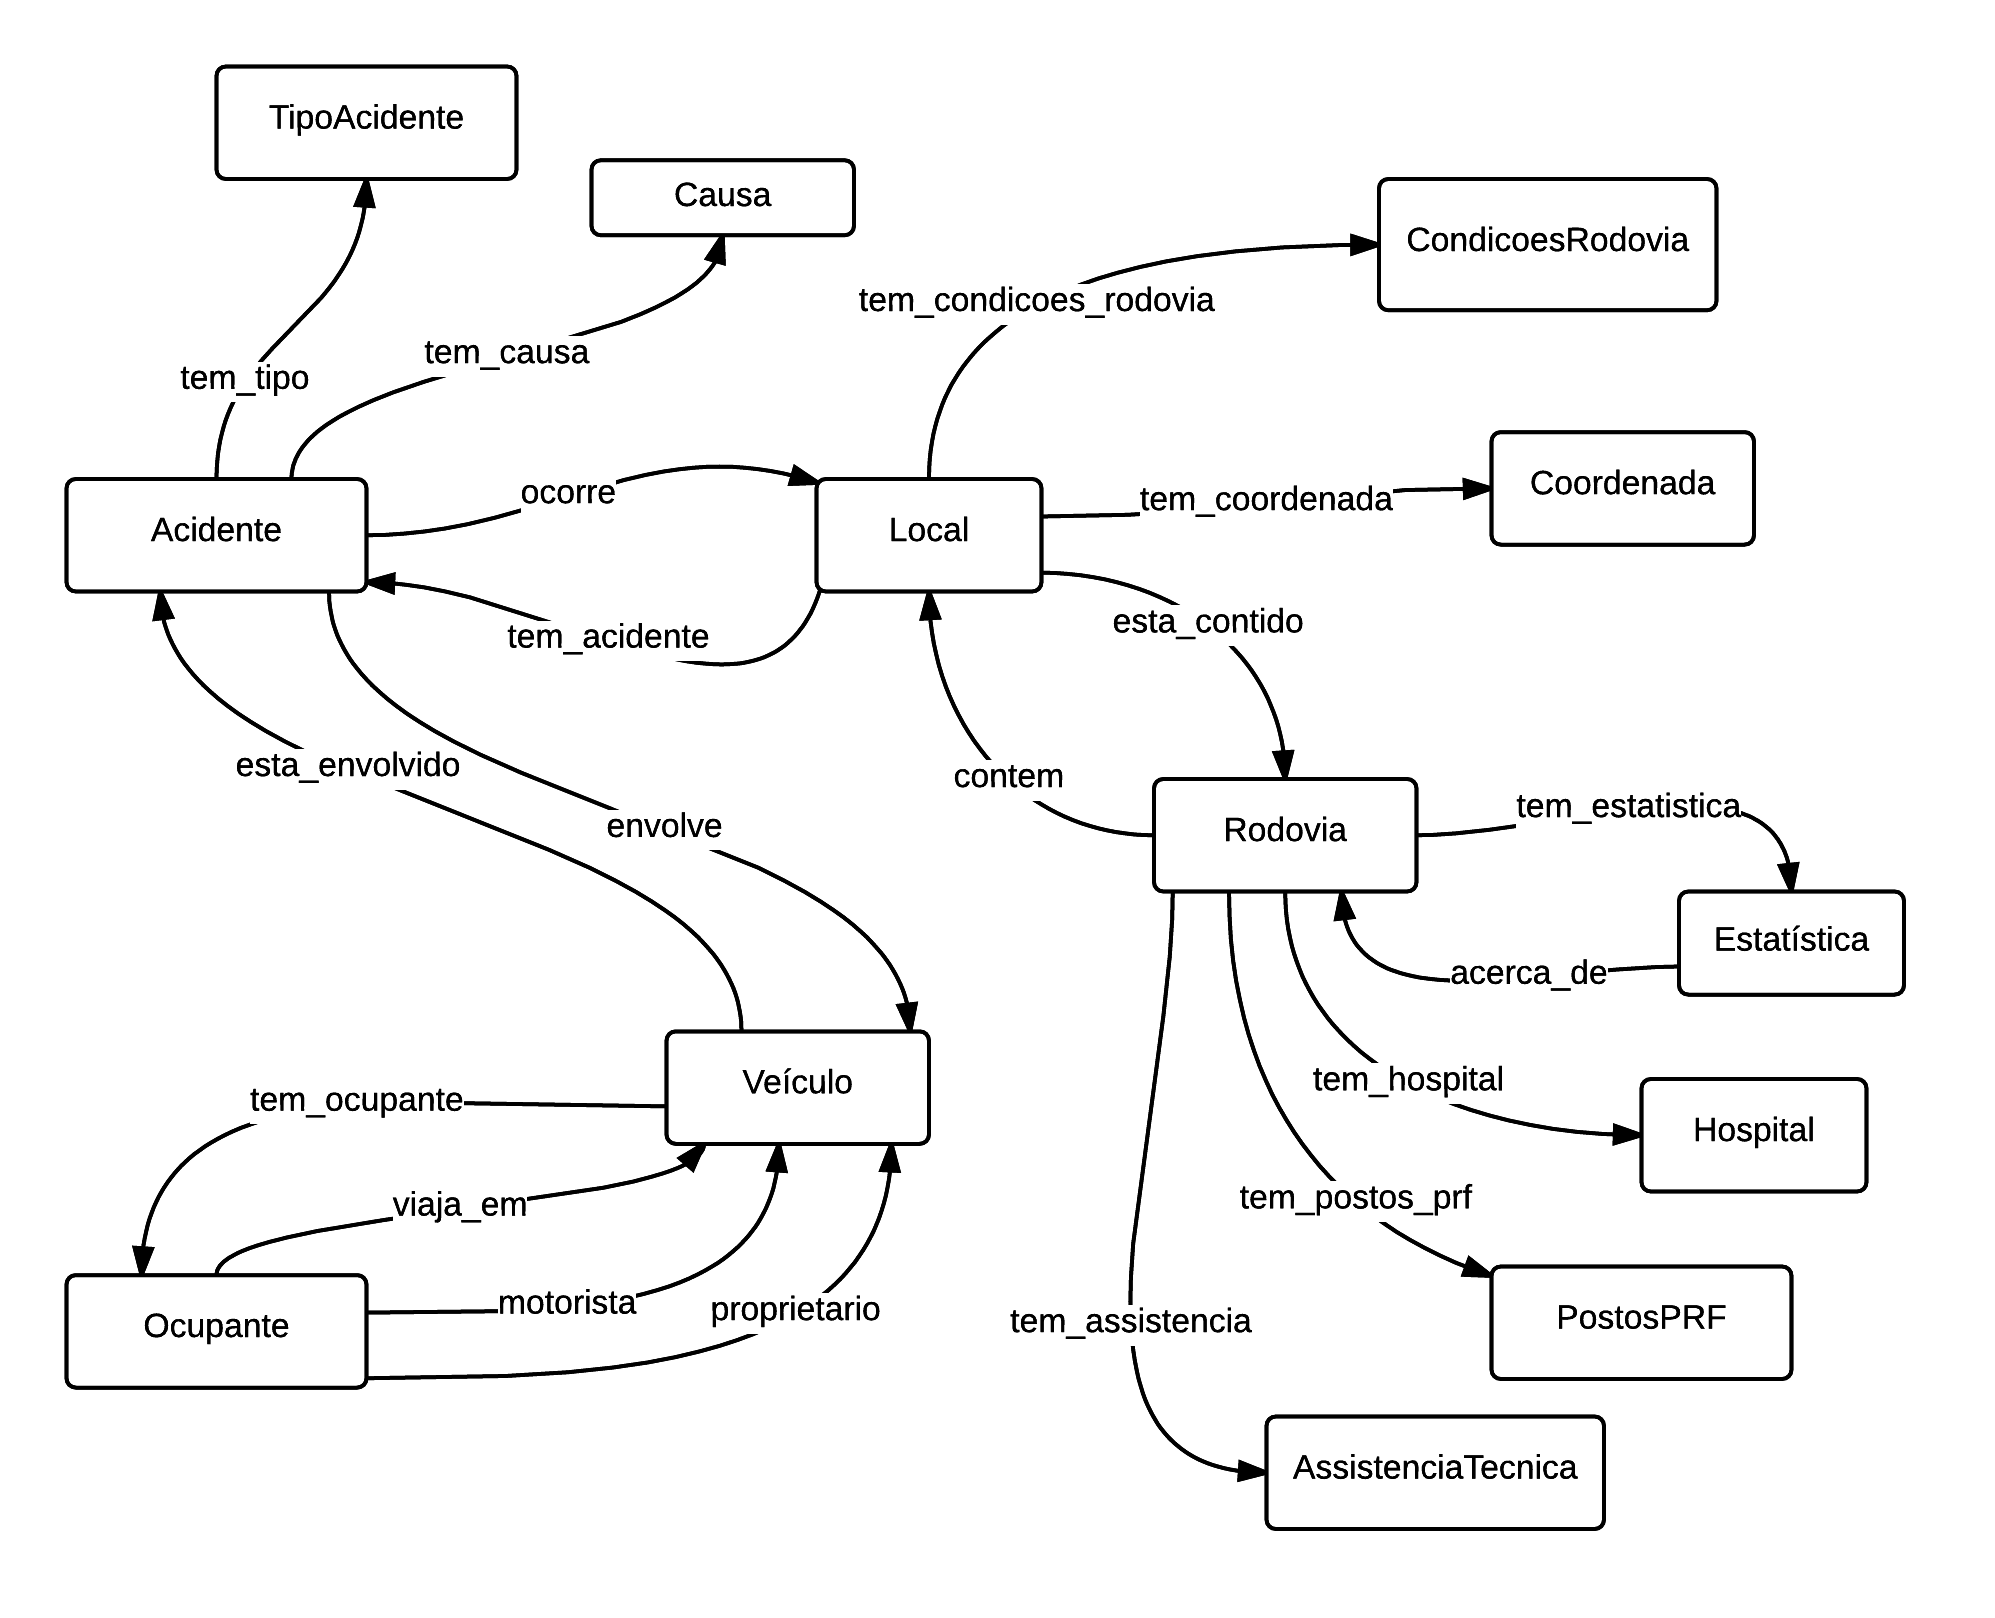
\includegraphics[scale = 0.4]{modelo_conceitual_ontologia.png}
	    \caption[Modelo conceitual da ontologia]{Modelo conceitual da ontologia a ser construída}
	    \label{fig:modelo_conceitual_ontologia}
	  \end{figure}
	  
	  O modelo conceitual apresentado se assemelha bastante com o padrão do grafo final que se obteria com a construção da
	  ontologia.
      
      \vfill
      \pagebreak
      \subsection{Atributos das classes}
	
	  Apesar de não estar descrito no modelo conceitual apresentado, por questão de organização, as classes levantadas
	  possuem atributos importantes que serão descritos nesse tópico.
	  
	  Para a definição dos atributos das classes foram considerados alguns atributos definidos no modelo de dados atual
	  da PRF.
	  
	  % Classe Acidente
\subsubsection{\textbf{Acidente}}

  A classe Acidente pode ser considerada como a classe central para a aplicação e para a ontologia,
  uma vez que todas as outras classes estão relacionadas a um acidente ocorrido.
  
    \begin{table*}[!h]
    \centering
    \begin{tabular}{p{0.15\linewidth}p{0.2\linewidth}p{0.5\linewidth}}
      \hline
      \textbf{Classe} & \textbf{Atributo} & \textbf{Descrição}\\
      \hline
	Acidente & data\_acidente & Data da ocorrência do acidente\\
		 & hora\_acidente & Horário da ocorrência do acidente\\
		 & danos\_causados & Descrição dos danos causados pelo acidente\\
      \hline
    \end{tabular}
    \caption{Atributos da classe Acidente}
    \label{tab:attr_acidente}
    \end{table*}
    
% Classe Veículo
\subsubsection{\textbf{Veículo}}

  A classe Veículo representa os veículos envolvidos em um acidente.
  
    \begin{table*}[!h]
    \centering
    \begin{tabular}{p{0.15\linewidth}p{0.22\linewidth}p{0.5\linewidth}}
      \hline
      \textbf{Classe} & \textbf{Atributo} & \textbf{Descrição}\\
      \hline
	Veiculo & tipo\_veiculo & Tipo do veículo (Ex.: Hatch, sedan, caminhonete)\\
		& modelo\_veiculo & Modelo do veículo\\
		& ano\_veiculo & Ano do veículo\\		
		& km\_veiculo & Quilometragem do veículo no momento do acidente\\
		& defeitos\_veiculo & Defeitos encontrados no veículo no momento do acidente\\
		& quantidade\_pessoas & Quantidade de pessoas dentro do veículo no momento do acidente\\
      \hline
    \end{tabular}
    \caption{Atributos da classe Veículo}
    \label{tab:attr_veiculo}
    \end{table*}

% \vfill
% \pagebreak

% Classe Ocupante
\subsubsection{\textbf{Ocupante}}

  A classe Ocupante representa as pessoas que podem estar dentro de um veículo no momento do acidente.
  
    \begin{table*}[!h]
    \centering
    \begin{tabular}{p{0.15\linewidth}p{0.23\linewidth}p{0.5\linewidth}}
      \hline
      \textbf{Classe} & \textbf{Atributo} & \textbf{Descrição}\\
      \hline
	Ocupante & sexo & Modelo do veículo\\
		 & idade\_pessoa & Idade da pessoa\\
		 & usava\_cinto & Indica se o ocupante do veículo estava usando o cinto de segurança\\
		 & estado\_mental* & Indica o estado mental do motorista no momento do acidente\\
		 & sob\_efeito\_toxicos* & Indica se o motorista estava sob efeito de tóxicos no momento do acidente\\
		 & uf\_cnh\_motorista* & UF da CNH do motorista\\
      \hline
    \end{tabular}
    *Atributos específicos para instâncias com a relação 'motorista'.

    \caption{Atributos da classe Ocupante}
    \label{tab:attr_ocupante}
    \end{table*}
    
% Classe Local
\subsubsection{\textbf{Local}}

  A classe Local representa o local, dentro de uma rodovia, no qual um acidente ocorreu.
  
    \begin{table*}[!h]
    \centering
    \begin{tabular}{p{0.15\linewidth}p{0.23\linewidth}p{0.5\linewidth}}
      \hline
      \textbf{Classe} & \textbf{Atributo} & \textbf{Descrição}\\
      \hline
	Local & latitude & Latitude em que ocorreu o acidente\\
	      & longitude & Longitude em que ocorreu o acidente\\
	      & km\_rodovia & Indica em qual quilômetro da rodovia ocorreu o acidente\\
	      & ponto\_referencia & Indica um ponto de referência próximo ao local do acidente\\
	      & regiao\_urbana & Indica se a área do acidente é uma região urbana\\
	      & volume\_trafego & Indica o volume de tráfego na região\\
      \hline
    \end{tabular}
    \caption{Atributos da classe Local}
    \label{tab:attr_local}
    \end{table*}

% \vfill
% \pagebreak
    
% Classe Rodovia
\subsubsection{\textbf{Rodovia}}

  A classe Rodovia representa as rodovias federais brasileiras. No domínio da aplicação, todo acidente ocorre em uma rodovia.
  
    \begin{table*}[!h]
    \centering
    \begin{tabular}{p{0.15\linewidth}p{0.23\linewidth}p{0.5\linewidth}}
      \hline
      \textbf{Classe} & \textbf{Atributo} & \textbf{Descrição}\\
      \hline
	Rodovia & nome\_rodovia & Nome da rodovia (Ex.: BR-060)\\
		& extensao\_rodovia & Indica o tamanho da rodovia\\
		& estado\_rodovia & Identifica quais estados brasileiros que a rodovia percorre\\
		& posto\_prf & Identifica um posto da PRF ao longo da rodovia\\
      \hline
    \end{tabular}
    \caption{Atributos da classe Rodovia}
    \label{tab:attr_rodovia}
    \end{table*}

% Classe Estatística    
\subsubsection{\textbf{Estatística}}

  A classe Estatística representa as estatísticas que pode se inferir sobre os acidentes ocorridos em uma rodovia.
  
    \begin{table*}[!h]
    \centering
    \begin{tabular}{p{0.15\linewidth}p{0.23\linewidth}p{0.5\linewidth}}
      \hline
      \textbf{Classe} & \textbf{Atributo} & \textbf{Descrição}\\
      \hline
	Estatística & nome\_estatistica & Nome da estatística\\
		    & tipo\_estatistica & Indica o tipo da estatística\\
		    & valor\_estatistica & Identifica o valor da estatística\\
		    & desvio\_padrao & Indica o desvio padrão da estatística calculada\\
		    & data\_calculo & Indica a data em que foi calculada aquela estatística\\
      \hline
    \end{tabular}
    \caption{Atributos da classe Estatística}
    \label{tab:attr_estatistica}
    \end{table*}    

% Classe Causa    
\subsubsection{\textbf{Causa}}

  A classe Causa representa as possíveis causas de uma acidente. Para trabalhos futuros, pretende-se especializar esta classe 
  nas diferentes causas de acidentes existentes ou, se possível, utilizar uma ontologia de causas de acidentes.
  
    \begin{table*}[!h]
    \centering
    \begin{tabular}{p{0.15\linewidth}p{0.23\linewidth}p{0.5\linewidth}}
      \hline
      \textbf{Classe} & \textbf{Atributo} & \textbf{Descrição}\\
      \hline
	Causa & descricao\_causa & Descrição da causa do acidente\\
	      & tipo\_causa & Indica o tipo da causa de acidente (Ex.: Falha técnica, condição da pista, etc.)\\
	      & periculosidade & Identifica o grau de periculosidade da causa\\
      \hline
    \end{tabular}
    \caption{Atributos da classe Causa}
    \label{tab:attr_causa}
    \end{table*}      
    
% Classe TipoAcidente    
\subsubsection{\textbf{TipoAcidente}}

  A classe TipoAcidente representa os tipos de acidentes que podem estar relacionados a determinado acidente.
  
    \begin{table*}[!h]
    \centering
    \begin{tabular}{p{0.15\linewidth}p{0.23\linewidth}p{0.5\linewidth}}
      \hline
      \textbf{Classe} & \textbf{Atributo} & \textbf{Descrição}\\
      \hline
	TipoAcidente & nome\_tipo & Indica o nome do tipo de acidente\\
		     & descricao\_tipo & Descrição do tipo de acidente\\
      \hline
    \end{tabular}
    \caption{Atributos da classe TipoAcidente}
    \label{tab:attr_tipo_acidente}
    \end{table*}
    
% Classe PostosPRF    
\subsubsection{\textbf{PostoPRF}}

  A classe PostoPRF representa os os postos da PRF que podem estar localizados em uma rodovia.
  Os postos da PRF localizam-se ao longo das rodovias, o que os classificam como um tipo de local definido na
  classe Local. Logo, a classe PostoPRF possuem os mesmos atributos da classe Local, como latitude e longitude,
  e mais os seguintes:
  
    \begin{table*}[!h]
    \centering
    \begin{tabular}{p{0.15\linewidth}p{0.23\linewidth}p{0.5\linewidth}}
      \hline
      \textbf{Classe} & \textbf{Atributo} & \textbf{Descrição}\\
      \hline
	PostoPRF & nome\_posto & Indica o nome do posto da PRF (Ex.: 10º posto da Polícia Rodoviária Federal)\\
		 & encarregado\_posto & Indica o nome do chefe responsável pelo posto da PRF\\
		 & telefone & Indica o número de telefone do posto da PRF\\
		 & email & Indica o endereço de \textit{e-mail} do posto da PRF\\
		 & detalhes\_posto & Informa detalhes sobre o posto da PRF (Ex.: Há local para pouso de aeronaves)\\
      \hline
    \end{tabular}
    \caption{Atributos da classe PostoPRF}
    \label{tab:attr_postoprf}
    \end{table*}
    
% Classe AssistenciaTecnica    
\subsubsection{\textbf{AssistenciaTecnica}}

  A classe AssistenciaTecnica representa entidades que possam oferecer algum serviço de assistência aos motoristas, localizadas 
  ao longo ou nas cidades mais próximas de uma rodovia.
  
    \begin{table*}[!h]
    \centering
    \begin{tabular}{p{0.15\linewidth}p{0.23\linewidth}p{0.5\linewidth}}
      \hline
      \textbf{Classe} & \textbf{Atributo} & \textbf{Descrição}\\
      \hline
	PostoPRF & nome\_assistencia & Indica o nome da unidade de assistência técnica\\
		 & tipo\_assistencia & Indica o tipo de assistência oferecida (Ex.: Borracharia)\\
		 & endereco & Indica o endereço da unidade de assistência técnica\\
		 & telefone & Indica o número de telefone da unidade de assistência técnica\\
      \hline
    \end{tabular}
    \caption{Atributos da classe PostoPRF}
    \label{tab:attr_postoprf}
    \end{table*}
    
% Classe Hospital    
\subsubsection{\textbf{Hospital}}

  A classe Hospital representa as unidades hospitalares localizadas próxima a uma rodovia. Para trabalhos futuros, pretende-se
  utilizar uma ontologia para a definição de hospitais.
  
    \begin{table*}[!h]
    \centering
    \begin{tabular}{p{0.15\linewidth}p{0.23\linewidth}p{0.5\linewidth}}
      \hline
      \textbf{Classe} & \textbf{Atributo} & \textbf{Descrição}\\
      \hline
	Hospital & nome\_hospital & Indica o nome do hospital\\
		 & especialidade & Indica qual a especialidade do hospital\\
		 & endereco & Indica o endereço do hospital\\
		 & telefone & Indica o número de telefone do hospital\\
      \hline
    \end{tabular}
    \caption{Atributos da classe Hospital}
    \label{tab:attr_hospital}
    \end{table*}
    
\vfill
      
      \pagebreak
      \subsection{Modelagem da ontologia no Protégé}
      
	As classes e propriedades definidas foram modeladas na ferramenta Protégé \footnotemark[2],
	de acordo com o modelo conceitual final	apresentado na Figura \ref{fig:modelo_conceitual_ontologia}.
	\footnotetext[2]{http://protege.stanford.edu/}
	
	As Figuras \ref{fig:classes_protege} e \ref{fig:propriedades_protege} apresentam, respectivamente, as classes e
	as propriedades que foram modeladas no Protégé.
	
	\begin{figure}[!htb]
	  \centering
	  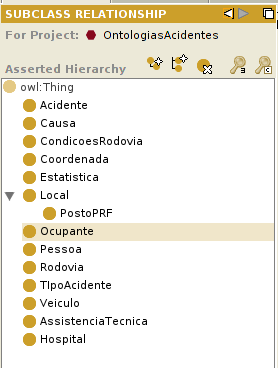
\includegraphics[scale = 0.55]{classes_wsm}
	  \caption[Classes modeladas no Protégé]{Classes modeladas no Protégé.}
	  \label{fig:classes_protege}
	\end{figure}
	
	\begin{figure}[!htb]
	  \centering
	  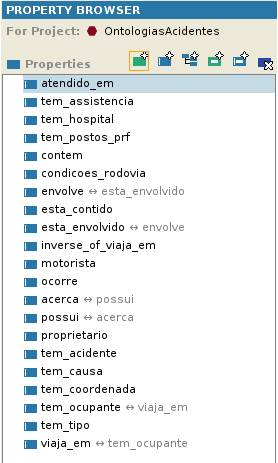
\includegraphics[scale = 0.6]{propriedades_classes_wsm}
	  \caption[Propriedades das classes modeladas no Protégé]{Propriedades das classes modeladas no Protégé.}
	  \label{fig:propriedades_protege}
	\end{figure}
	
      \pagebreak
      \section{Cronograma para Construção da Ontologia na Aplicação}

A aplicação da ontologia no software envolvem algumas mudanças estruturais na arquitetura e
na refatoração de algumas funcionalidades, como uma busca no banco de dados por um acidente por 
exemplo. Desta forma, a equipe técnica definiu a construção da ontologia na aplicação como um projeto
separado, com cronograma próprio, integrado com o cronograma geral do projeto.
O objetivo é encarar a construção como uma mudança de requisitos, estudando o impacto e analisando
as implicações do uso da ontologia dentro da ferramenta, com base nas métricas de qualidade previamente 
definidas. 

\begin{figure}[h]
	\centering
	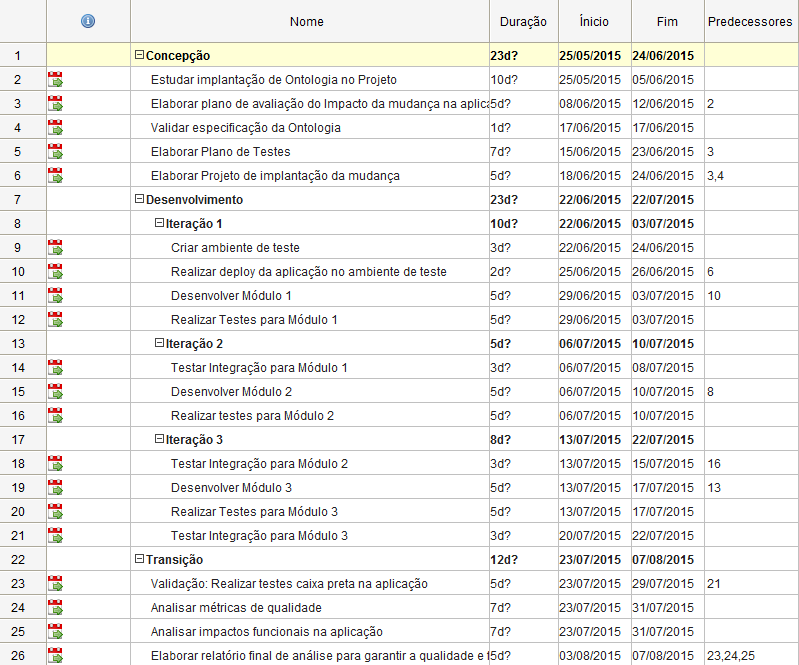
\includegraphics[scale=0.6]{Figuras/cronograma_construcao_ontologia.png}
\end{figure}

\pagebreak

Tabela – Cronograma de Construção da Ontologia na Aplicação

\subsection{Esforço versus Impacto da Construção}

Com base no cronograma, é necessário observar que existe um grau de esforço que será empregado,
com custos inerentes ao processo de software. A mudança mais relevante é o uso do framework \textit{Active RDF} \footnotemark[1], no lugar do \textit{Active Record} que faz deixa transparente o acesso de dados da camada \textit{Model} com o banco de dados. 

A hipótese é de que \textbf{os benefícios da aplicação dessa mudança sejam relevantes a ponto de justificar o custo inerente à mudança do software}. Para analisar a hipótese e refletir sobre suas implicações, foi necessário calcular os custos de produção. O valor considerado pela equipe técnica da hora de um aluno da UnB foi de dez reais e sessenta e cinco centavos, adicionados os valores de consumo de energia e mensalidade da internet. O valor do custo total foi baseado numa rotina de trabalho de 5 horas semanais, durante 58 dias, conforme a divisão de trabalho do cronograma.

O custo total da implementação da mudança na aplicação \textit{Pé na Estrada} ficou em 3088,50 R\$ . Esse valor, divido pelos 58 dias de trabalho, caracterizam 53,25 R\$ por dia de trabalho.

\begin{figure}[h] 
	\centering % para centralizarmos a figura
	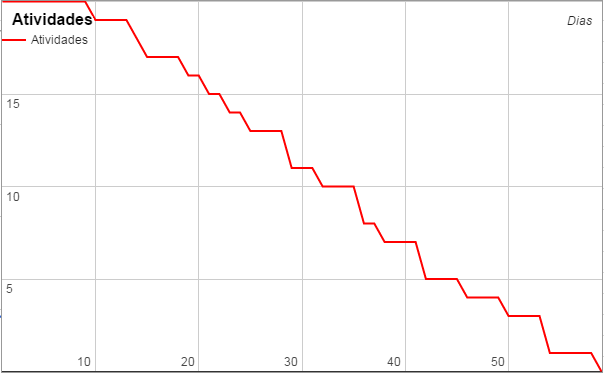
\includegraphics[scale=0.6]{Figuras/grafico_atividades.png} % leia abaixo

\end{figure}

Figura - Burndown das Atividades

\begin{figure}[h] 
	\centering % para centralizarmos a figura
	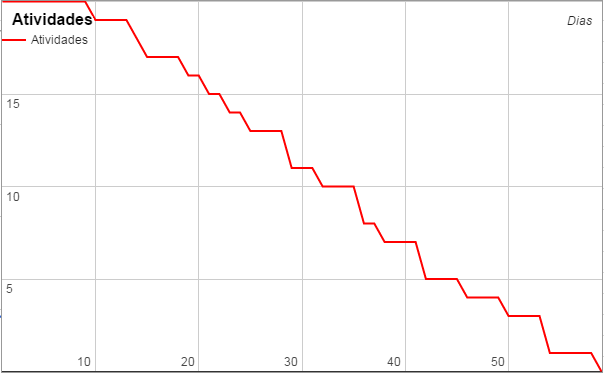
\includegraphics[scale=0.6]{Figuras/grafico_atividades.png} % leia abaixo
	
\end{figure}

Gráfico - Gráfico de Custo Planejado

A discussão sobre os resultados e sobre a hipótese levantada nesse seção serão discutidas no tópico \textbf{Resultados Esperados}. 
